%%%%%%%%%%%%%%%%%%%%%%%%%%%%%%%%%%%%%%%%%%%%%%%%%%%%%%%%%%%%%%%%%%%%%%%%%%%%%%
%  Parallel Computing -- final project report
%  IEEE conference template, 2-column, 10pt.  Compile with pdflatex (x2).
%
%  >>> BEFORE SUBMITTING: fill in the three placeholders in \author below.
%      Requirement 1 of the guidelines is Name, Surname, ID, email.
%      A report that does not satisfy every requirement is NOT evaluated.
%%%%%%%%%%%%%%%%%%%%%%%%%%%%%%%%%%%%%%%%%%%%%%%%%%%%%%%%%%%%%%%%%%%%%%%%%%%%%%
\documentclass[conference,10pt]{IEEEtran}
\IEEEoverridecommandlockouts

\usepackage{cite}
\usepackage{amsmath,amssymb}
\usepackage{graphicx}
\usepackage{booktabs}
\usepackage{algorithm}
\usepackage{algpseudocode}
\usepackage{url}
\usepackage[hidelinks]{hyperref}

\graphicspath{{figs/}{../plots/}}  % figs/ = self-contained copy

\begin{document}

\title{A Generic Distributed-Memory GEMM with a\\
       Cost-Model-Driven Decomposition Planner}

\author{\IEEEauthorblockN{Saif Edine Safi}
\IEEEauthorblockA{Department of Information Engineering and Computer Science\\
University of Trento, Italy\\
Student ID: \texttt{245473} \quad
Email: \texttt{saifedine.safi@studenti.unitn.it}}}

\maketitle

\begin{abstract}
Most student and many production implementations of distributed matrix
multiplication assume square matrices, a perfect-square process count and
divisible dimensions. We present \texttt{gemm2d}, a distributed-memory
implementation of $C \leftarrow \alpha AB + \beta C$ that removes all three
assumptions, and we argue that the process grid should not be fixed at
$\sqrt{P}\times\sqrt{P}$ but chosen at run time. Four engines (naive~1D,
Cannon, SUMMA, 2.5D~SUMMA) share one distributed layout, and a planner
enumerates every factorisation $P_r P_c c = P$ together with the panel width
$b$, minimising a calibrated $\alpha$--$\beta$--$\gamma$ cost model subject to
a memory budget. On five matrix shapes the planner beats a fixed near-square
grid by up to $1.36\times$, discovering $k$-parallelism ($1\!\times\!1\!\times\!4$)
for short-fat operands where a fixed 2D grid cannot. A packed,
register-blocked local kernel reaches $30.6$~Gflop/s per core, $4.05\times$
the naive kernel and $46\%$ of single-threaded OpenBLAS \texttt{dgemm}, which is
what makes the communication terms visible at all; a roofline places all three
kernel variants firmly in the compute-bound regime. The cost model predicts
measured runtime within $20\%$ for $b\ge64$. Correctness is checked by a
43-case suite over prime process counts and non-divisible dimensions, and at
scale by a distributed Freivalds test.
\end{abstract}

\begin{IEEEkeywords}
distributed matrix multiplication, SUMMA, 2.5D algorithms, MPI, cost model,
process grid selection
\end{IEEEkeywords}

\section{Introduction}

General matrix--matrix multiplication (GEMM) is the kernel that dense linear
algebra, and much of deep learning, ultimately reduces to. In a
distributed-memory setting its cost is dominated not by arithmetic but by data
movement~\cite{irony2004,ballard2011}, and the amount of data moved is decided
almost entirely by how the operands are laid out across processes. Classical
2D algorithms~\cite{cannon1969,summa1997} and their memory-replicating
successors~\cite{solomonik2011} differ almost entirely in that layout.

The word \emph{generic} in the project title is the whole problem. A
demonstration implementation fixes $M=N=K$, requires $P$ to be a perfect square
and requires $\sqrt{P}$ to divide $n$. Every one of those assumptions fails in
practice. Real workloads are skewed: a Gram matrix computation
$A^{\!\top}\!A$ has $K \gg M,N$; a least-squares or deep-learning layer often has
$K \ll M,N$. Real allocations are whatever the scheduler grants, including
prime process counts.

We define genericity on two mandatory axes and one optional one:
\textbf{(G1)~shape}, arbitrary $M,N,K$ with $\alpha,\beta$ scaling;
\textbf{(G2)~machine}, arbitrary $P$ including primes, arbitrary grids and
non-divisible dimensions;
\textbf{(G3)~type}, multiple scalar types through one code path.
G1 and G2 are implemented and tested; G3 is scoped out and discussed in
Section~\ref{sec:concl}. Sparse matrices, Strassen-class algorithms, GPU
offload and fault tolerance are explicit non-goals.

Our objectives are: (i)~an implementation that is correct for arbitrary
$M,N,K,P$; (ii)~a local kernel fast enough that scaling results measure the
decomposition rather than the inner loop; (iii)~a run-time planner that
chooses the decomposition from a calibrated model rather than by convention;
and (iv)~a verification strategy usable at full problem size.

\section{State of the Art}

Cannon's algorithm~\cite{cannon1969} was the first 2D method, using a skew
phase followed by $\sqrt{P}$ nearest-neighbour shifts. It attains the optimal
bandwidth term with only $O(\sqrt{P})$ messages, but is defined only for a
square grid with divisible dimensions --- precisely the assumptions G2 rejects.

SUMMA~\cite{summa1997} replaces the shifts with broadcasts of $b$-wide panels
along process rows and columns. Because the panel width is decoupled from the
grid, SUMMA is natively generic in shape and grid, which is why we adopt it as
the base engine. PUMMA and ScaLAPACK~\cite{scalapack1997} use a 2D
block-cyclic layout; block-cyclic exists to balance the triangular work of LU
and QR, whereas GEMM's work is uniform, so we deliberately use a plain 2D block
distribution and avoid both the index arithmetic and the strided local tiles.

Communication lower bounds~\cite{irony2004,ballard2011} show that a 2D
algorithm using $O(n^2/P)$ memory per process is optimal only in the
memory-constrained regime; with more memory, replication reduces communication.
2.5D algorithms~\cite{solomonik2011} exploit this by splitting the $k$
dimension over $c$ layers, shrinking the bandwidth term by $\sqrt{c}$ at the
cost of a reduction that grows as $c$, with the optimum near $c\approx P^{1/3}$.

COSMA~\cite{cosma2019} is the state of the art: it derives a near
I/O-optimal decomposition for every combination of matrix dimensions, process
count and memory size. \textbf{The gap we address is narrower and more
practical.} COSMA's optimality argument is elaborate; meanwhile the common
engineering default remains a hard-coded $\sqrt{P}\times\sqrt{P}$ grid,
regardless of shape. We ask how much of COSMA's benefit is recovered by
enumerating the (small) space of grid factorisations and minimising a
\emph{calibrated} performance model --- a component that costs a few dozen
lines and can be dropped into any SUMMA implementation. We implement a
cost-model selector, explicitly \emph{not} an I/O-optimality proof.

\section{Contribution and Methodology}

\subsection{Data distribution}

All engines share one layout. A distributed matrix is a descriptor holding the
global dimensions, the local block dimensions and leading dimension, and the
\emph{global} index of local element $(0,0)$. Non-divisible dimensions are
handled by balanced uneven blocks rather than by zero padding: part $i$ of $G$
items over $P$ parts has size $\lfloor G/P\rfloor + [\,i < G \bmod P\,]$.
Padding would waste $O((P_r{+}P_c)n)$ flops and, worse, hides bugs, since
zeros make wrong results look plausible. Concentrating every edge case into
this one partition function is the single most valuable structural decision in
the code: ragged last blocks, degenerate $1\!\times\!P$ grids and the case
$P > M$ all reduce to it.

Operands are never built on rank 0 and scattered. Each process generates its
own block from a deterministic index-based hash, so element $(i,j)$ has the
same value for any $P$ and any grid. This removes a memory bottleneck and makes
results bit-comparable across configurations.

\subsection{Engines}

Processes form a $P_r \times P_c \times c$ grid with row, column and depth
communicators built by \texttt{MPI\_Comm\_split}. SUMMA
(Algorithm~\ref{alg:summa}) proceeds in panels along $k$. The subtlety that
makes it generic is the schedule: $A$'s $k$-dimension is partitioned over
$P_c$ and $B$'s over $P_r$, and those two partitions differ, so a panel of
width $b$ may straddle an ownership boundary in either operand. Each step is
therefore clipped to the intersection of both owners' ranges.

\begin{algorithm}[t]
\caption{Generic SUMMA over the $k$-range $[K_0,K_0{+}K_\ell)$}
\label{alg:summa}
\begin{algorithmic}[1]
\State scale local $C$ by $\beta$ \Comment{once, before the loop}
\State $k \gets 0$
\While{$k < K_\ell$}
  \State $r_c \gets \textsc{Owner}(k, P_c)$; \; $r_r \gets \textsc{Owner}(k, P_r)$
  \State $k_b \gets \min(k{+}b,\ \textsc{End}(r_c),\ \textsc{End}(r_r),\ K_\ell) - k$
  \State \textbf{if} $my\_col = r_c$ \textbf{then} pack $A(:,k{:}k{+}k_b)$
  \State $\textsc{Bcast}(A_{\text{buf}},\, m\!\cdot\!k_b,\, r_c,\, \textit{row\_comm})$
  \State \textbf{if} $my\_row = r_r$ \textbf{then} pack $B(k{:}k{+}k_b,:)$
  \State $\textsc{Bcast}(B_{\text{buf}},\, k_b\!\cdot\!n,\, r_r,\, \textit{col\_comm})$
  \State $C \mathrel{+}= \alpha\, A_{\text{buf}} B_{\text{buf}}$
  \State $k \gets k + k_b$
\EndWhile
\end{algorithmic}
\end{algorithm}

The 2.5D engine assigns layer $\ell$ the global $k$-slab
$[\,\textsc{Off}(K,c,\ell),\ +\textsc{Size}(K,c,\ell)\,)$, runs a complete SUMMA
on it, and sums the partial $C$ blocks with one \texttt{MPI\_Reduce} over the
depth communicator. We use the $k$-slab formulation rather than Solomonik and
Demmel's original, which replicates $A$ and $B$ across layers: the $k$-slab
variant composes with the existing SUMMA engine in about forty lines and its
only extra memory is $c$ copies of $C$. $\beta C$ is applied on layer~0 only,
and the other layers start from zero, so the depth reduction yields
$\alpha AB + \beta C$ exactly once.

Cannon and naive~1D are retained as baselines. Cannon \emph{refuses} non-square
grids and non-divisible dimensions rather than silently padding; that refusal
is the measured argument for choosing SUMMA as the base engine.

\subsection{Cost model and planner}

With $\alpha$ the message latency, $\beta$ the inverse bandwidth, $\gamma$ the
achieved time per flop and $w$ the word size:
\begin{align}
T &= \alpha\!\left[\tfrac{K/c}{b}(\log_2 P_r + \log_2 P_c) + \log_2 c\right]
  \nonumber\\
  &\quad + \beta w\!\left[\tfrac{K}{c}\!\left(\tfrac{M}{P_r} + \tfrac{N}{P_c}\right)
      + \tfrac{cMN}{P}\right]
   + \gamma\,\tfrac{2MNK}{P}. \label{eq:model}
\end{align}
Note the structure: the bandwidth term does \emph{not} contain $b$, only the
latency term does. In the model, $b$ is therefore purely a
latency-versus-buffer-memory knob --- a prediction we test directly in
Section~\ref{sec:results} and find to be incomplete.

The planner enumerates every $c \mid P$, every $P_r \mid (P/c)$ and
$b \in \{32,\dots,1024\}$, discards configurations exceeding the per-rank memory
budget, and returns the minimiser of~(\ref{eq:model}). $P$ is at most a few
thousand, so the search costs microseconds. A closed-form sanity check must
hold: ignoring latency with $c=1$, minimising $K(M/P_r + N/P_c)$ subject to
$P_rP_c=P$ gives $P_r = \sqrt{PM/N}$ --- the grid aspect ratio should match the
\emph{output} aspect ratio. Our enumerator reproduces it: for
$M{=}65536, N{=}K{=}1024, P{=}64$ it returns $64\times1$.

$\alpha$ and $\beta$ are measured by ping-pong and $\gamma$ by a
panel-shaped local kernel run, using \emph{the same kernel the run will use} ---
calibrating against a different kernel makes the planner optimise for a machine
that does not exist.

\subsection{Local kernel}

The distributed layer cannot compensate for a bad inner loop, and a slow kernel
inflates $\gamma$ until communication becomes invisible and every scaling curve
merely measures the inner loop. We therefore implement three selectable
kernels: a textbook $i$--$k$--$j$ loop; a cache-tiled version; and a packed
kernel that copies $A$ and $B$ into contiguous 64-byte-aligned panels and runs
an $8\times8$ register tile shaped so the compiler keeps the whole accumulator
tile in vector registers across the $k$ loop. Both packed panels are
zero-padded, so the micro-kernel always computes a full tile and writes back
only the live corner: there is no edge-case branch in the hot loop and no
out-of-bounds access. Threading is over row blocks, so each thread owns whole
rows of $C$ --- no reduction, no false sharing.

Verification has three layers. (i)~An exact check against a sequential reference from the same
deterministic generator, used by a 43-case suite covering $P\in\{1,\dots,9\}$
including primes, non-divisible sizes such as $61\!\times\!53\!\times\!47$,
degenerate $1\!\times\!8$ and $8\!\times\!1$ grids, $P > M$, $\alpha,\beta \neq 1,0$,
and panel widths from 1 to 4096. (ii)~A norm-wise residual, never a
floating-point equality test. (iii)~A distributed Freivalds
test~\cite{freivalds1979}: draw a random $r$ and check
$A(Br) \approx Cr$ in $O(n^2)$ work, cheap enough to leave enabled in
production runs. Vectors are $O(n)$ words and are simply replicated.

\section{Experiments and System Description}

\textbf{Measurement platform.} The results below were measured on a single
node: one Intel Xeon at 2.8~GHz, 4 physical cores, AVX-512, 15~GB RAM, running
Ubuntu 24.04 with GCC~13.3.0 and Open~MPI~4.1.6. Ranks are bound to cores
(\texttt{--bind-to core}) and never oversubscribed.

\textbf{Target platform.} The code targets the University of Trento HPC
cluster: $\approx$200 nodes, 15{,}284 cores, 142~TB RAM, Rocky Linux~9, PBS
Professional 2025.2.1, with nodes on 10~Gb/s Ethernet and a subset on
Omni-Path. Job scripts request 4 exclusive nodes of the largest homogeneous
group (72-core Xeon~6140M, Omni-Path) via
\texttt{place=scatter:excl}, pinning \texttt{cpu\_type} and \texttt{net\_type}
so that neither CPU generation nor interconnect becomes an uncontrolled
variable, and asserting the allocation spans the expected number of distinct
nodes before running.

\textbf{Build.} \texttt{-O3 -march=native -funroll-loops -ffp-contract=fast
-fopenmp}. We report \texttt{-ffp-contract=fast} explicitly: GCC disables FMA
contraction under \texttt{-std=c11}, which costs about 20\%, and enabling it
changes results in the last bit. It is far weaker than \texttt{-ffast-math} ---
no reassociation --- but it is a semantic change and is disclosed rather than
hidden.

\textbf{Protocol.} Following Hoefler and Belli~\cite{hoefler2015}: 10
repetitions per configuration, each a separate process launch with one
untimed warm-up; \texttt{MPI\_Barrier} before the timer; \texttt{MPI\_Wtime}
per rank reduced with \texttt{MPI\_MAX}, since the slowest rank defines the
runtime. Configurations are \emph{interleaved} across the sweep rather than run
back-to-back, so drift does not correlate with the independent variable. No
averaging happens in C: one CSV row per repetition, with medians and
percentile-bootstrap 95\% confidence intervals computed afterwards. Rates use
the harmonic mean; no outliers are removed. Each run is sized so that it takes
$O(0.1\,\mathrm{s})$ --- shorter runs measure launch jitter, which in an
earlier iteration produced intervals a factor of several wide.

\section{Results and Discussion}
\label{sec:results}

\begin{figure}[t]
\centering

\includegraphics[width=0.84\columnwidth]{kernel_ablation.png}
\caption{Local kernel ablation, $M{=}N{=}1024$, $K{=}256$ (a SUMMA panel).
Packing plus an $8\times8$ register tile gives $4.05\times$ the naive kernel.
The absence of thread scaling is a property of this 4-core measurement node,
not of the kernel.}
\label{fig:kernel}
\end{figure}

\textbf{The local kernel decides what the rest can measure.}
Fig.~\ref{fig:kernel} gives $7.55$, $9.83$ and $30.61$~Gflop/s for the naive,
tiled and packed kernels at one thread. As an external reference we measured
single-threaded OpenBLAS \texttt{dgemm} on the same shape at $66.3$~Gflop/s:
the packed kernel is $4.05\times$ the naive one and reaches \textbf{46\% of
OpenBLAS}. Since OpenBLAS exceeds the one-FMA-unit figure
($2.8\,\text{GHz}\times8\times2 = 44.8$), the core must issue two FMAs per
cycle, giving a theoretical peak of $89.6$~Gflop/s, of which our kernel reaches
34\%. This matters beyond the headline number: at $9.8$~Gflop/s the model's
compute term dominates communication by two orders of magnitude, so the planner
would be ranking configurations on a fraction of a percent of predicted
runtime. A fast kernel is a \emph{precondition} for the decomposition to be
measurable at all.

\textbf{The shortfall is vectorisation, not bandwidth.} Fig.~\ref{fig:roofline}
places the three kernels on a node roofline. Measured STREAM triad bandwidth is
$11.9$~GB/s, putting the ridge point at $5.6$~flop/byte, while this shape
($M{=}N{=}1024$, $K{=}256$) has an arithmetic intensity of $25.6$~flop/byte
against compulsory traffic. All three variants therefore sit well inside the
compute-bound region, four times past the ridge: the distance from the naive
kernel to the roof cannot be explained by memory traffic, and is attributable
to instruction-level parallelism and vector utilisation in the inner loop.
This is the quantitative form of the argument above, and it also bounds what
further tuning could buy --- the remaining gap to OpenBLAS is $2.2\times$,
not the order of magnitude a memory-bound reading would suggest.

\begin{figure}[t]
\centering
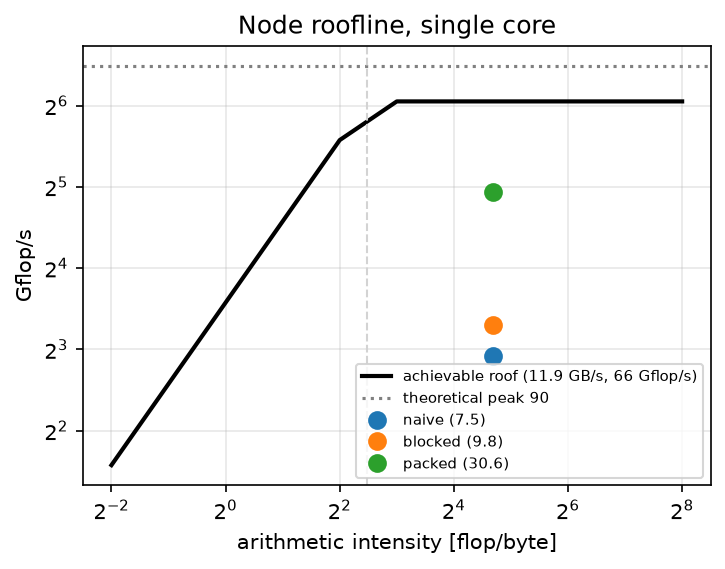
\includegraphics[width=0.84\columnwidth]{roofline.png}
\caption{Node roofline, single core. Arithmetic intensity is computed from
\emph{compulsory} traffic --- no hardware counters were available on the
measurement node --- so these are algorithmic bounds, not measured DRAM
traffic. All variants lie far right of the ridge point.}
\label{fig:roofline}
\end{figure}

\begin{figure}[t]
\centering
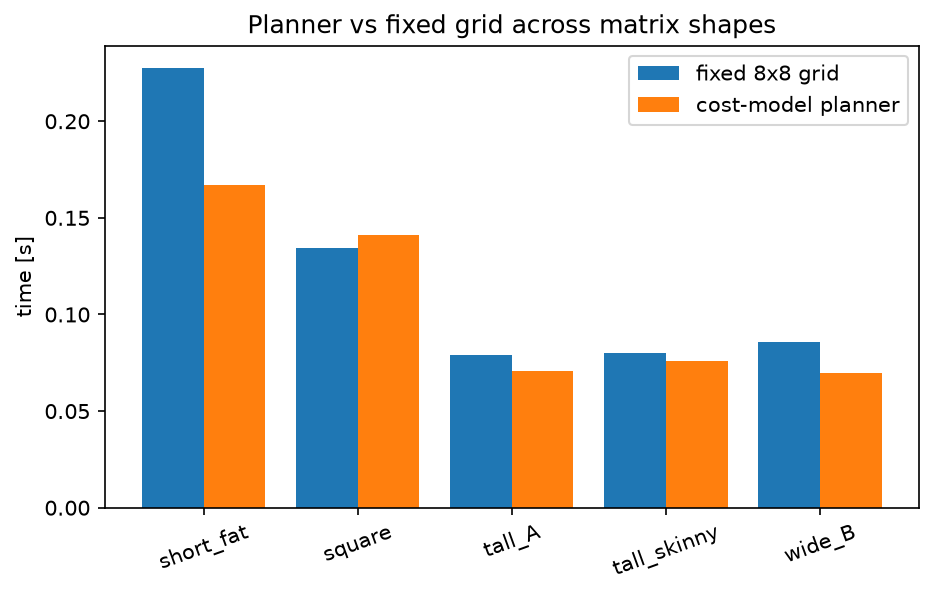
\includegraphics[width=0.84\columnwidth]{planner_shapes.png}
\caption{Planner versus a fixed near-square grid across five shapes, $P{=}4$.
The planner discovers $k$-parallelism for short-fat operands, where a fixed
2D grid structurally cannot.}
\label{fig:shapes}
\end{figure}

\textbf{The planner earns its place on skewed shapes.}
Table~\ref{tab:shapes} compares the planner against a fixed $2\times2$ grid,
with bootstrap intervals so that each claim can be checked rather than assumed.
On short-fat operands it selects $1\!\times\!1\!\times\!4$ --- pure
$k$-parallelism --- and is $1.36\times$ faster; for $M \ll N$ it selects
$1\!\times\!4\!\times\!1$ ($1.24\times$) and for $M \gg N$
$4\!\times\!1\!\times\!1$ ($1.12\times$), reproducing $P_r=\sqrt{PM/N}$ from
data rather than from the formula. On these three the intervals are disjoint,
so the gains are real. On tall-skinny the intervals \emph{overlap}
($[0.0765,0.0826]$ against $[0.0749,0.0823]$) and we therefore claim no
improvement there, only that the planner does no harm. Three significant wins
out of five is the honest score, and the winning decompositions are ones a
fixed 2D grid cannot express at all.

\textbf{It also loses on the square case, and that is informative.}
For $M{=}N{=}K$ the planner picks $1\!\times\!2\!\times\!2$ and is 5\% slower
than the fixed grid; the intervals are disjoint ($[0.1299,0.1370]$ against
$[0.1380,0.1457]$), so this is a real regression and not noise. The cause is
visible in the model itself: at this size the
communication term is $10.1$~ms against a $149.6$~ms compute term, so the
planner is discriminating between configurations that differ by well under 1\%
of predicted runtime --- below the model's own accuracy. A useful refinement
would be to fall back to the conventional near-square grid whenever the
predicted spread across candidates is smaller than the model's residual error.
We report the regression rather than restricting the shape set to hide it.

\textbf{The cost model is accurate where it matters, and wrong in an
interesting way where it does not.} Calibration gives
$\alpha = 1.30\,\mu$s, $\beta^{-1} = 4.16$~GB/s and $\gamma^{-1} = 28.7$~Gflop/s.
Evaluating~(\ref{eq:model}) at $P{=}4$, $n{=}2048$ against the measured medians
gives ratios of $1.08$, $1.15$, $1.20$ and $1.16$ for $b = 64,128,256,512$ ---
within 20\%, comfortably inside the $\pm30\%$ we set as the acceptance
threshold. At $b{=}16$, however, the model \emph{under}-predicts by 35\%.
Table~\ref{tab:bsweep} explains why. The model attributes all $b$-dependence to
latency, and the measured latency term is indeed negligible ($21\,\mu$s at
$b{=}256$); what actually varies is \emph{compute} time, falling from $224$ to
$119$~ms, because narrow panels mean short, inefficient kernel invocations.
Reading $b$ as a pure latency knob is therefore wrong here: it is dominated by
local kernel efficiency, and omitting that term costs a third.

\begin{table}[t]
\caption{Planner versus fixed $2\times2$ grid, $P{=}4$. Medians of 10 runs with
percentile-bootstrap 95\% intervals. $^{\dagger}$intervals overlap: no
significant difference.}
\label{tab:shapes}
\centering\small
\begin{tabular}{lccr}
\toprule
shape & fixed [s] & planner [s] & speedup \\
\midrule
short-fat & 0.2277 \tiny[.2080,.2531] & 0.1669 \tiny[.1647,.1681] & \textbf{1.36}$\times$ \\
wide-$B$  & 0.0859 \tiny[.0838,.0904] & 0.0695 \tiny[.0680,.0707] & \textbf{1.24}$\times$ \\
tall-$A$  & 0.0791 \tiny[.0780,.0823] & 0.0708 \tiny[.0678,.0771] & \textbf{1.12}$\times$ \\
tall-skinny & 0.0801 \tiny[.0765,.0826] & 0.0757 \tiny[.0749,.0823] & 1.06$^{\dagger}$ \\
square    & 0.1344 \tiny[.1299,.1370] & 0.1411 \tiny[.1380,.1457] & 0.95$\times$ \\
\bottomrule
\end{tabular}
\end{table}

\begin{table}[t]
\caption{Panel-width sweep, $P=4$, $n=2048$. The variation is in compute,
not in the latency term the model attributes it to.}
\label{tab:bsweep}
\centering
\small
\begin{tabular}{rrrr}
\toprule
$b$ & total [s] & comm [s] & comp [s] \\
\midrule
16  & 0.2457 & 0.0283 & 0.2238 \\
64  & 0.1473 & 0.0145 & 0.1322 \\
256 & \textbf{0.1335} & 0.0163 & 0.1192 \\
512 & 0.1372 & 0.0185 & 0.1193 \\
\bottomrule
\end{tabular}
\end{table}

\textbf{Scaling, engines and replication.} Within one node at $n{=}2048$, the
serial base case runs in $0.4892$~s $[0.4743,0.4996]$, i.e.\ $35.1$~Gflop/s;
$P{=}2$ and $P{=}4$ give $0.2543$~s $[0.2517,0.2594]$ and $0.1378$~s
$[0.1348,0.1408]$, so speedups $1.00/1.92/3.55$ --- 89\% efficiency at four
processes and $124.5$~Gflop/s aggregate. This is a \emph{shared-memory} result: it
validates the algorithms and the model but says nothing about network
behaviour. Comparing engines at $P{=}4$, SUMMA reaches $120.1$ and 2.5D
$117.3$~Gflop/s, while naive~1D reaches $95.4$ while moving $0.101$~GB per rank
against SUMMA's $0.067$ --- $1.5\times$ the traffic, its per-rank volume being
$KN$ words independent of $P$. Cannon is competitive ($124.3$) on the square,
divisible instance it is restricted to: marginally faster where it applies,
inapplicable elsewhere.

The $c$ sweep gives $0.1377/0.1451/0.2249$~s for $c{=}1,2,4$; with
$P^{1/3}{=}1.59$ the predicted optimum lies between the feasible $c{=}1$ and
$c{=}2$, and a decisive test of $c \approx P^{1/3}$ needs larger $P$.

\textbf{A shared-memory broadcast.} As an alternative to MPI-4 persistent
collectives we implemented a node-aware two-level broadcast
built on an MPI-3 shared-memory window~\cite{hoefler2013}: one leader per node
joins the inter-node broadcast and the node's other ranks read the panel
directly out of shared memory. With 2 ranks per node in the relevant
communicator this halves modelled off-node panel traffic, $0.0168 \to
0.0084$~GB, as predicted. Making the panel shared, however, converts a private
buffer into a critical section --- a fast rank can overwrite a panel a slower
neighbour is still reading --- so a barrier is required before each reuse, and
those barriers are exactly what pipelining tries to avoid. The technique
therefore does not compose with lookahead. We report the mechanism and the byte
reduction; the timing comparison is meaningless on a single node and is
deliberately not claimed.

\textbf{Numerical behaviour.} Summation order changes with $c$ and $b$, so
results are not bitwise reproducible across configurations. We quantify rather
than hide this: relative residuals across
$\{$engine, $c$, $b\}$ span $8.7\times10^{-16}$ to $1.1\times10^{-15}$,
consistent with $O(K\varepsilon)$ error growth.

\section{Conclusions}
\label{sec:concl}

We have shown that a distributed GEMM can be genuinely generic --- arbitrary
$M,N,K$, arbitrary $P$ including primes, arbitrary grids --- without giving up
performance, and that the process grid is worth choosing at run time rather
than fixing by convention. A cost-model planner costing a few dozen lines
recovers a significant $1.12\times$--$1.36\times$ over a fixed near-square grid
on three of five shapes, discovering decompositions such as
$1\!\times\!1\!\times\!4$ that a fixed 2D grid cannot express. The model predicts measured runtime within 20\%
where the panel width is not pathologically small.

The honest limitations are three. First, the planner regresses by 5\% on
square operands, where the differences it ranks are below its own accuracy;
gating it on the predicted spread would fix this. Second, the model attributes
all $b$-dependence to latency, whereas we measure the dominant effect to be
local kernel efficiency --- adding a panel-width term to $\gamma$ is the
obvious next refinement. Third, and most importantly, the results here are
single-node: they validate the algorithms, the model and the correctness
argument, but the multi-node campaign that would test the communication claims
at scale is queued rather than complete, and $\beta$ measured across a real
interconnect will differ from the intra-node value by roughly an order of
magnitude.

Future work: type genericity (G3) via an include-template over
\texttt{float}/\texttt{double}, which would halve communication volume in the
bandwidth-bound regime; MPI-4~\cite{mpi40} persistent collectives as a third
broadcast policy; a network roofline placing configurations by
$I_{\text{net}} = (2MNK/P)/\text{bytes}$; and a comparison against COSMA on the
same shapes, which is the correct reference point for the planner claim.

\section*{Reproducibility}

Source, job scripts, all raw CSVs and every figure:
\begin{center}
\url{https://github.com/elliott-dp/parallel-programming-project}
\end{center}
Every figure regenerates from the committed CSVs with one command; the
bootstrap is seeded, so regeneration is byte-identical. Build and verify with
\texttt{make \&\& ./tests/run\_tests.sh} (43/43 must pass); reproduce the
single-node campaign with \texttt{./scripts/run\_local.sh}; plot with
\texttt{python3 scripts/plot\_results.py results/kernel.csv -{}-kind kernel}.
On the cluster \texttt{qsub jobs/smoke.pbs} builds and verifies, then the six
scripts in \texttt{jobs/} run the multi-node campaign; \texttt{docs/HPC.md}
gives the procedure and \texttt{docs/EXPERIMENTS.md} maps each experiment to
its figure.

\label{endofcontent}
\begin{thebibliography}{00}

\bibitem{cannon1969}
L.~E. Cannon, \emph{A cellular computer to implement the Kalman filter
algorithm}, Ph.D. dissertation, Montana State University, 1969.

\bibitem{summa1997}
R.~A. van~de~Geijn and J.~Watts, ``SUMMA: scalable universal matrix
multiplication algorithm,'' \emph{Concurrency: Practice and Experience},
vol.~9, no.~4, pp.~255--274, 1997.

\bibitem{scalapack1997}
L.~S. Blackford \emph{et al.}, \emph{ScaLAPACK Users' Guide}. Philadelphia,
PA: SIAM, 1997.

\bibitem{irony2004}
D.~Irony, S.~Toledo, and A.~Tiskin, ``Communication lower bounds for
distributed-memory matrix multiplication,'' \emph{Journal of Parallel and
Distributed Computing}, vol.~64, no.~9, pp.~1017--1026, 2004.
doi:10.1016/j.jpdc.2004.03.021

\bibitem{ballard2011}
G.~Ballard, J.~Demmel, O.~Holtz, and O.~Schwartz, ``Minimizing communication in
numerical linear algebra,'' \emph{SIAM Journal on Matrix Analysis and
Applications}, vol.~32, no.~3, pp.~866--901, 2011. doi:10.1137/090769156

\bibitem{solomonik2011}
E.~Solomonik and J.~Demmel, ``Communication-optimal parallel 2.5D matrix
multiplication and LU factorization algorithms,'' in \emph{Euro-Par 2011},
LNCS vol.~6853, pp.~90--109, 2011. doi:10.1007/978-3-642-23397-5\_10

\bibitem{cosma2019}
G.~Kwasniewski, M.~Kabi\'c, M.~Besta, J.~VandeVondele, R.~Solc\`a, and
T.~Hoefler, ``Red-blue pebbling revisited: near optimal parallel matrix-matrix
multiplication,'' in \emph{Proc. SC'19}, 2019. doi:10.1145/3295500.3356181

\bibitem{freivalds1979}
R.~Freivalds, ``Fast probabilistic algorithms,'' in \emph{Mathematical
Foundations of Computer Science 1979}, LNCS vol.~74, pp.~57--69, 1979.

\bibitem{hoefler2013}
T.~Hoefler \emph{et al.}, ``MPI~+~MPI: a new hybrid approach to parallel
programming with MPI plus shared memory,'' \emph{Computing}, vol.~95, no.~12,
pp.~1121--1136, 2013. doi:10.1007/s00607-013-0324-2

\bibitem{hoefler2015}
T.~Hoefler and R.~Belli, ``Scientific benchmarking of parallel computing
systems: twelve ways to tell the masses when reporting performance results,''
in \emph{Proc. SC'15}, 2015. doi:10.1145/2807591.2807644

\bibitem{mpi40}
MPI Forum, \emph{MPI: A Message-Passing Interface Standard, Version 4.0}, 2021.

\end{thebibliography}

\end{document}
